\chapter{Specific requirements}

\section{External Interface Requirements}
\subsection{User Interfaces}
The following mockups serve as guideline for the application, used by individuals, and the web application, used by third parties. The final product design may differ from these mockups but the functions provided has to be the same.


\begin{figure}[H]
\centering
\begin{minipage}{.5\textwidth}
  \centering
  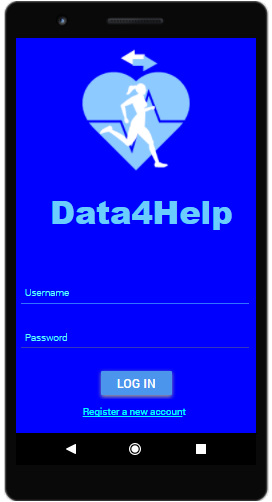
\includegraphics[width=5cm,height=9cm]{resources/Screen/Individuallogin.png}
  \captionof{figure}{App Login screen}
  \label{fig:App Login}
\end{minipage}%
\begin{minipage}{.5\textwidth}
  \centering
  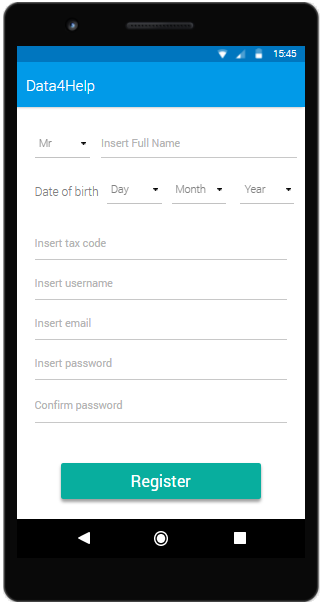
\includegraphics[width=5cm,height=9cm]{resources/Screen/RegistrationIndividual.png}
  \captionof{figure}{Registration screen}
  \label{fig:App Registration}
\end{minipage}
\end{figure}


\begin{figure}[H]
\centering
\begin{minipage}{.5\textwidth}
  \centering
  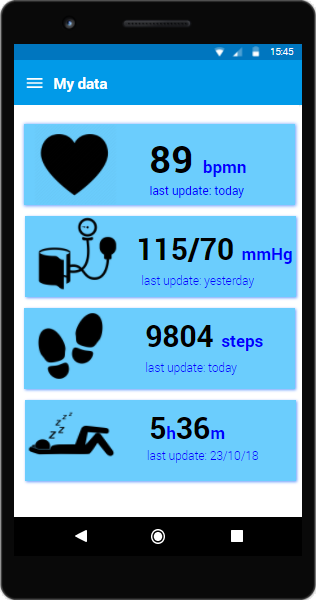
\includegraphics[width=5cm,height=9cm]{resources/Screen/IndividualMyData.png}
  \captionof{figure}{App My data screen}
  \label{fig:App data homepage}
\end{minipage}%
\begin{minipage}{.5\textwidth}
  \centering
  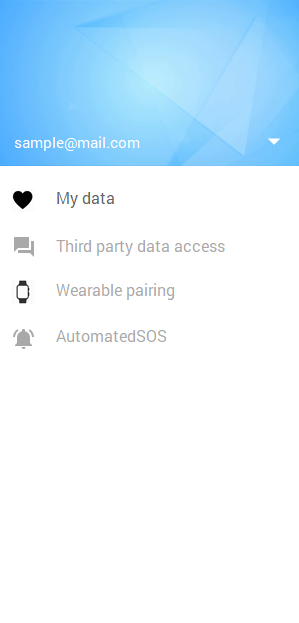
\includegraphics[width=5cm,height=9cm]{resources/Screen/menuindividual.png}
  \captionof{figure}{App side menu screen}
  \label{fig:App Side menu}
\end{minipage}
\end{figure}


\begin{figure}[H]
\centering
\begin{minipage}{.5\textwidth}
  \centering
  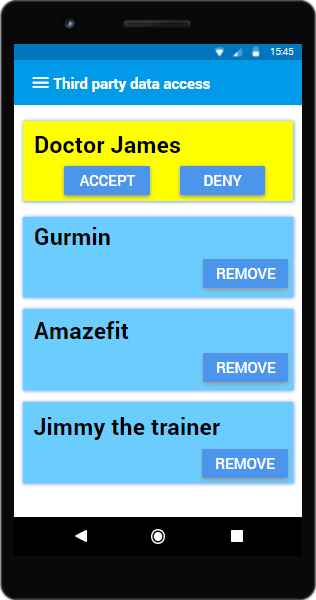
\includegraphics[width=5cm,height=9cm]{resources/Screen/ThirdPartyManagementIndividual.png}
  \captionof{figure}{App Third Party management screen}
  \label{fig:App ThirdParty Management}
\end{minipage}%
\begin{minipage}{.5\textwidth}
  \centering
  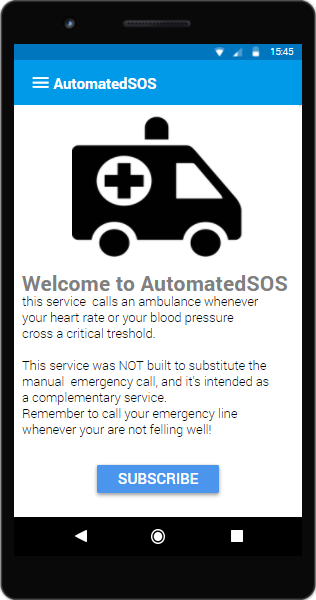
\includegraphics[width=5cm,height=9cm]{resources/Screen/AutomatedSOSIndividual.png}
  \captionof{figure}{App AutomatedSOS screen}
  \label{fig:App AutomatedSOS}
\end{minipage}
\end{figure}

\begin{figure}[H]
\centering
  \fbox{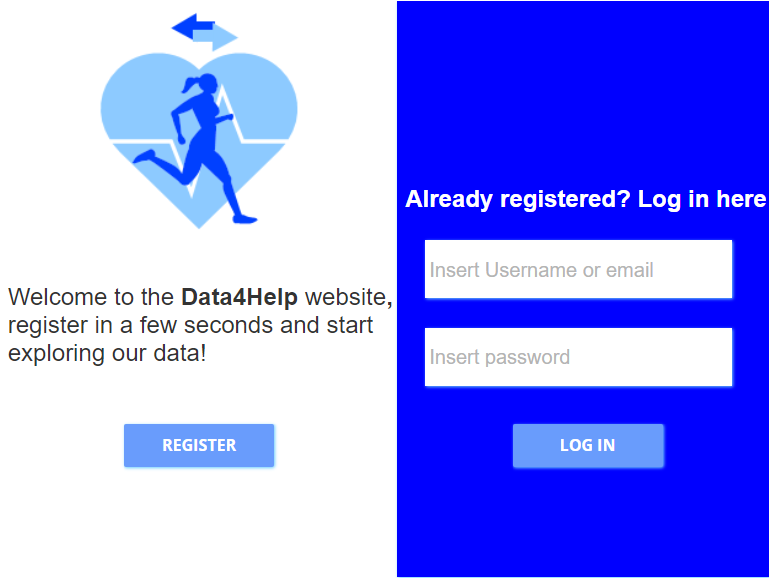
\includegraphics[width=12cm,height=9cm]{resources/Screen/ThirdPartyLogin.png}}
   \captionof{figure}{WebApp Home screen}
  \label{fig:WebApp Log in}
\end{figure}

\begin{figure}[H]
\centering
  \fbox{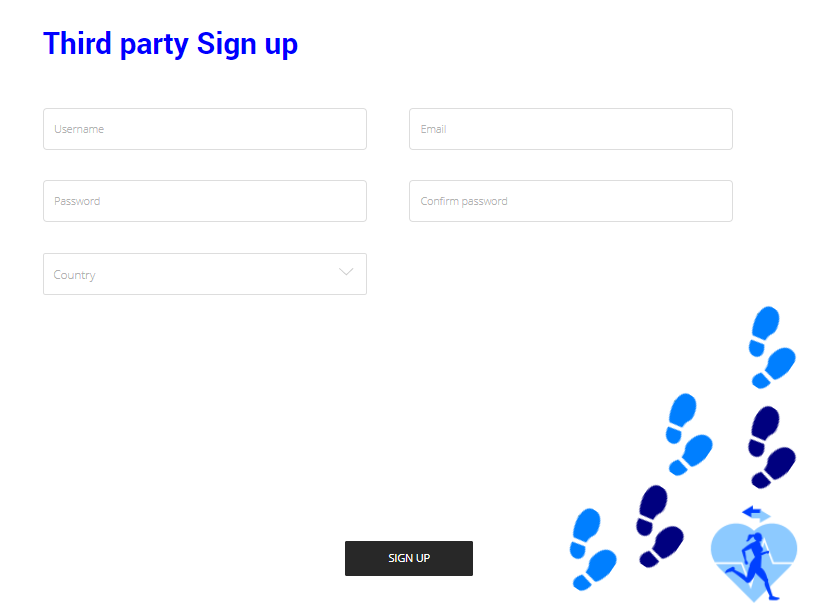
\includegraphics[width=12cm,height=9cm]{resources/Screen/ThirdPartySignup.png}}
   \captionof{figure}{WebApp Sign Up screen}
  \label{fig:WebApp SignUp}
\end{figure}

\begin{figure}[H]
\centering
  \fbox{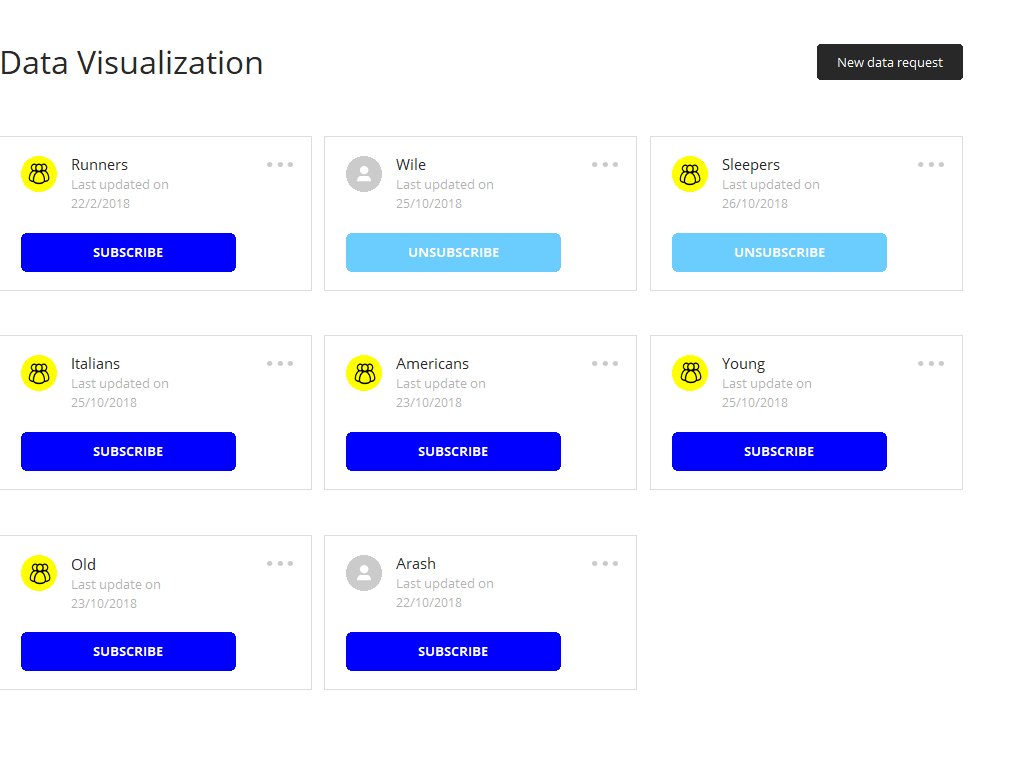
\includegraphics[width=12cm,height=9cm]{resources/Screen/DataVisualization.png}}
   \captionof{figure}{WebApp Data visualization screen}
  \label{fig:WebApp data visualization}
\end{figure}


\begin{figure}[H]
\centering
 \fbox{ 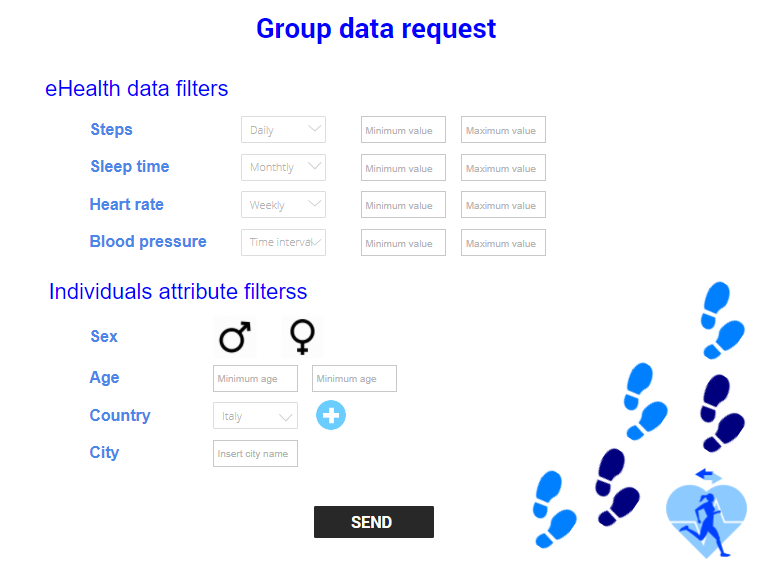
\includegraphics[width=12cm,height=9cm]{resources/Screen/Groupdatarequest.png}}
  \caption{WebApp Group data request}
  \label{fig:WebApp GroupData Request}
\end{figure}


\begin{figure}[H]
\centering
  \fbox{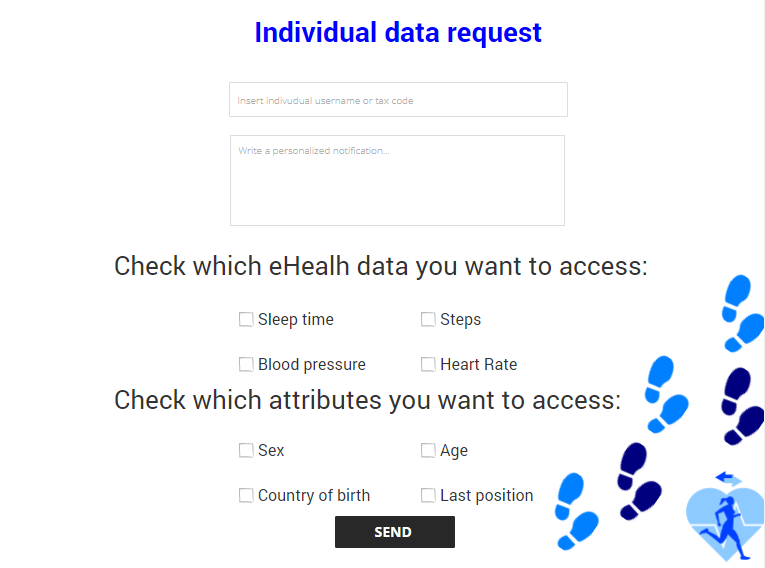
\includegraphics[width=12cm,height=9cm]{resources/Screen/individualdatarequest.png}}
  \caption{WebApp Individual data request}
  \label{fig:WebApp Individual data request}
\end{figure}


\begin{figure}[H]
\centering
  \fbox{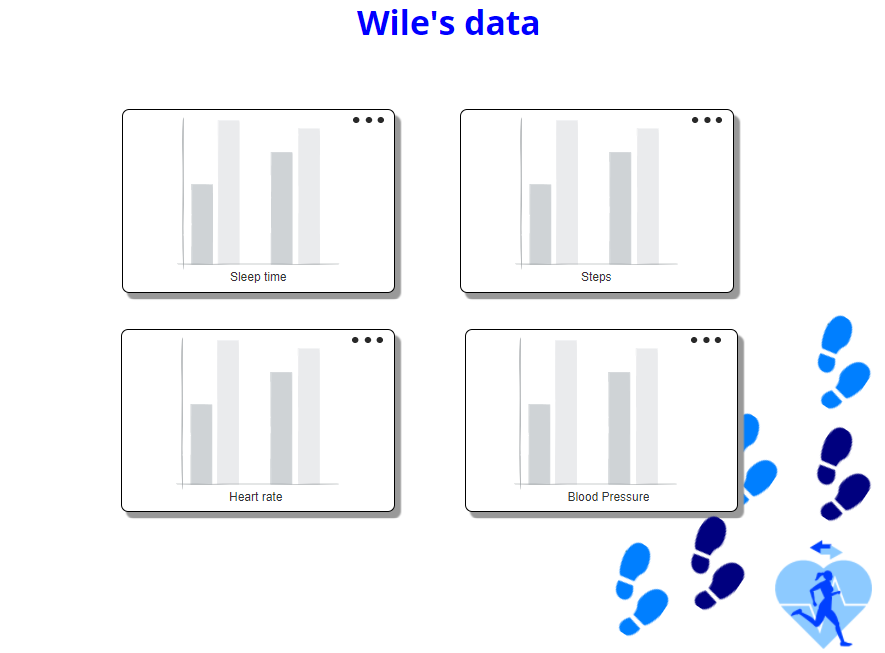
\includegraphics[width=12cm,height=9cm]{resources/Screen/individualdatavisualization.png}}
  \caption{Specific Data screen}
  \label{fig:WebApp Specific data screen}
\end{figure}

\subsection{Hardware Interfaces}
Data4Help is an application that can be accessed in two ways, based on the typology of the users:
\begin{itemize}
\item Individuals must access to the application through a supported smartphone with working GPS, bluetooth.
\item Third parties must access to the application through a compatible web browser with any kind of device. It is suggested, but not necessary to use a device with at least a 10 inches screen to have the best experience using the application.
\end{itemize}
Data4Help doesn't need any specific hardware interface, all its features will be reachable through the provided software applications.








\subsection{Software Interfaces}
In order to guarantee a quick development Data4Help system will use the following external software services:
\begin{itemize}
\item Ambulance call service API: for each country, where the AutomatedSOS service will be enabled, these APIs will be needed in order to implement the automatic call.
\item DBMS : this service will be used to manage all users data and satisfy third party queries.
\item Location Services: these services will be used to pick the individual position. His position will be used to enrich with more details the eHealth data and for the AutomatedSOS service.
\end{itemize}

\subsection{Communication Interfaces}
The smartphone application and the web application will both use HTTP to ensure a connection with Data4Help system.
The communication between the individuals' smartphone application and the wearable will use instead the bluetooth protocol.

\section{Scenarios}
\subsection{Scenario 1}

Rebecca has worked very hard in the last months and she has been a long stressful period. Recently she had to skip several working days because she didn't feel very well. 
She consulted her doctor John who didn't notice anything alarming.
John then discovered Data4Help and he thought that it could have been useful to monitor the health status of Rebecca on daily basis for the next weeks.
Then, John asked Rebecca to register to Data4Help and to use her smartwatch to collect some data.
Rebecca immediately registered to the service and accepted the request that John sent to her.
Now John can have a better look at his patient's health status and can make better diagnosis.


\subsection{Scenario 2}
Walter is a 75 years old man who lives alone in a small town.
His doctor has been monitoring him thanks to Data4Help because he has a cardiac disease.
Last week, Walter was at the supermarket and suddenly he fainted. Luckily, the store was crowded and therefore someone helped him and called an ambulance.
He is afraid it could happen again and because he lives alone, he decides to activate the AutomatedSOS service.


\subsection{Scenario 3}
FatBit is a startup that wants to launch its first wearable. To optimize their limited resources and to improve their ads, Fatbit's managers want to know which are the countries with healthier people, which one have the more active, and the average age of their potential consumers. Collecting this data it's not easy, especially when joining the market for the first time. Fortunately a new service, Data4Help, has just launched and its main features it's the distribution of eHealth data, organized according to different parameters, included the ones FatBit managers are interested in (age,location,steps taken daily).
Therefore FatBit's managers decide to register with a unique account as third party, and start their data analysis thanks to Data4Help.


\subsection{Scenario 4}
Wile is an engineering student who wants to get back in shape. He decides to join the gym and to buy a wearable to see its progress over time. Initially Wile is satisfied by his wearable and the built in application but later he starts noticing that more and more wearables with improved design and many new features are launching in the market. Wisely, he notices that the built in application collects the data only for the producer's devices and so if he wanted to change his wearable without losing data he were practically forced to buy a new watch from the same company. Therefore he decides to use Data4Help, allowing him to change his wearable with the one he likes the most without losing data.

\section{Functional Requirements}

\begin{enumerate}

\item[\textbf{[G\ref{g:Data}]}] \textbf{\goalData}

\begin{enumerate}

\item[][D\ref{d:ProvidingData}] {\domProvidingData}
\item[][D\ref{d:Internet}] {\domInternet}
\item[]\req{Users are able to login with the username and the password associated to their account.}{Login}
\item[]\req{Data4Help is able to pair with the user wearable.}{Pairing}
\item[]\req{Data4Help is able to download eHealth data from the individual's wearable.}{DownloadData}
\item[]\req{Individuals can upload their data through Data4Help app.}{Uploading}
\item[]\subreq{Data4Help is able to store the data provided by individuals.}{Storing}
\item[]\subreq{Data4Help is able to organize data provided by individuals.}{OrganizingData}



\end{enumerate}

\item[\textbf{[G\ref{g:GroupData}]}] \textbf{\goalGroupData}

\begin{enumerate}
\item[] [D\ref{d:Internet}] {\domInternet}
\item[] [R\ref{sr:Storing}] {\subreqStoring}
\item[] [R\ref{r:Login}] {\reqLogin}
\item[] [R\ref{sr:OrganizingData}] {\subreqOrganizingData}
\item[] \req{Third parties can formulate requests to access anonymized data of groups.}{Request}
\item[] \req{Third parties can apply filters on data while formulating their request for data of groups.}{Filtering}
\item[] \req{The system checks if the number of individuals in the group detected by the third party request is higher than 1000.}{PrivacyCheck}
\item[] \subreq{If the groups has 1000 or less individuals the system denies the request.}{DenyRequest}
\item[] \req{The system is able to distribute the requested data to the third party.}{Distribution}
\end{enumerate}

\item[\textbf{[G\ref{g:SpecData}]}] \textbf{\goalSpecData}
\begin{enumerate}

\item[] [D\ref{d:Internet}] {\domInternet}
\item[] [D\ref{d:SSNknown}] {\domSSNknown}
\item[] [R\ref{sr:Storing}] {\subreqStoring}
\item[] [R\ref{r:Login}] {\reqLogin}
\item[] [R\ref{sr:OrganizingData}] {\subreqOrganizingData}
\item[] \req{Third parties can formulate requests to access specific individual data, indicating the individual's TC or username.}{IndividualRequest}
\item[] \req{Third parties can apply filters on the type of data while formulating their request for individual data.}{IndividualFilters}
\item[] \req {Data4Help is able to forward the request to the individual specified by the third party.}{ReqForward}
\item[] \req{The individual to whom the request will be forwarded is able to reply.}{ReqReply}
\item[] \subreq{The system notifies the third party about the individual reply.}{ReqReply}
\item[] \req{The system can check if the individual has accepted the data access request by the third party.}{CheckReply}
\item[] [R\ref{r:Distribution}] {\reqDistribution}


\end{enumerate}

\item[\textbf{[G\ref{g:Notify}]}] \textbf{\goalNotify}

\begin{enumerate}
\item[] [D\ref{d:Internet}] {\domInternet}
\item[] [R\ref{r:Login}] {\reqLogin}
\item[] [R\ref{sr:Storing}] {\subreqStoring}
\item[] [R\ref{sr:OrganizingData}] {\subreqOrganizingData}
\item[] \req{Third parties can specify to be updated whenever new data of groups detected by their data requests, or observed individuals is gathered. The time interval between an update and the next one can be set by the third party, in a limit that goes from one hour to 1 year.}{DataSubscription}
\item[] \req{The system is able to update third parties with new data, respecting their preferences on the interval timing.}{SubScriptionUpdate}
\end{enumerate}

\item[\textbf{[G\ref{g:Rescue}]}] \textbf{\goalRescue}

\begin{enumerate}

\item[] [D\ref{d:Internet}] {\domInternet}
\item[] [R\ref{r:Login}] {\reqLogin}
\item[] \req{Individual can subscribe to the AutomatedSOS service.}{AutomatedSOS}
\item[] [R\ref{r:Pairing}] {\reqPairing}
\item[] [D\ref{d:OnePar}] {\domOnePar}
\item[] \req{The system is able to recognize if the wearable can measure at least a vital parameter.}{ParametersCheck}
\item[] \req{The system is able to continuously monitor individual vital parameters.}{Monitoring}
\item[] \req{If the wearable is disconnected the AutomatedSOS service is suspended, until the individual connects his wearable again.}{Disconnect}
\item[] [D\ref{d:Thresholds}]{\domThresholds}
\item[] [D\ref{d:Ambulance}]{\domAmbulance}
\item[] [D\ref{d:ProvidingData}]{\domProvidingData}
\item[] \req{Whenever a vital parameter cross its respective threshold, the system calls an ambulance in under 5 seconds, giving to the ambulance driver the location of the individual.}{AmbulanceCall}
\end{enumerate}

\item[\textbf{[G\ref{g:Privacy}]}] \textbf{\goalPrivacy}

\begin{enumerate}
\item[] [D\ref{d:Credential}] {\domCredential}
\item[] \req{The system doesn't allow third parties to access specific individuals data without first asking for their permission.}{Permission}
\item[] \req{The system stops to update third parties about new data whenever observed individuals decide to remove data access permissions, or whenever the number of individuals of an observed groups goes belove 1001.}{StopUpdates}
\item[] \req{Only users that know their username and password can access to their respective accounts}{AccountAccess}
\end{enumerate}
\end{enumerate}


\subsection{Use case diagram}
\begin{figure}[H]
  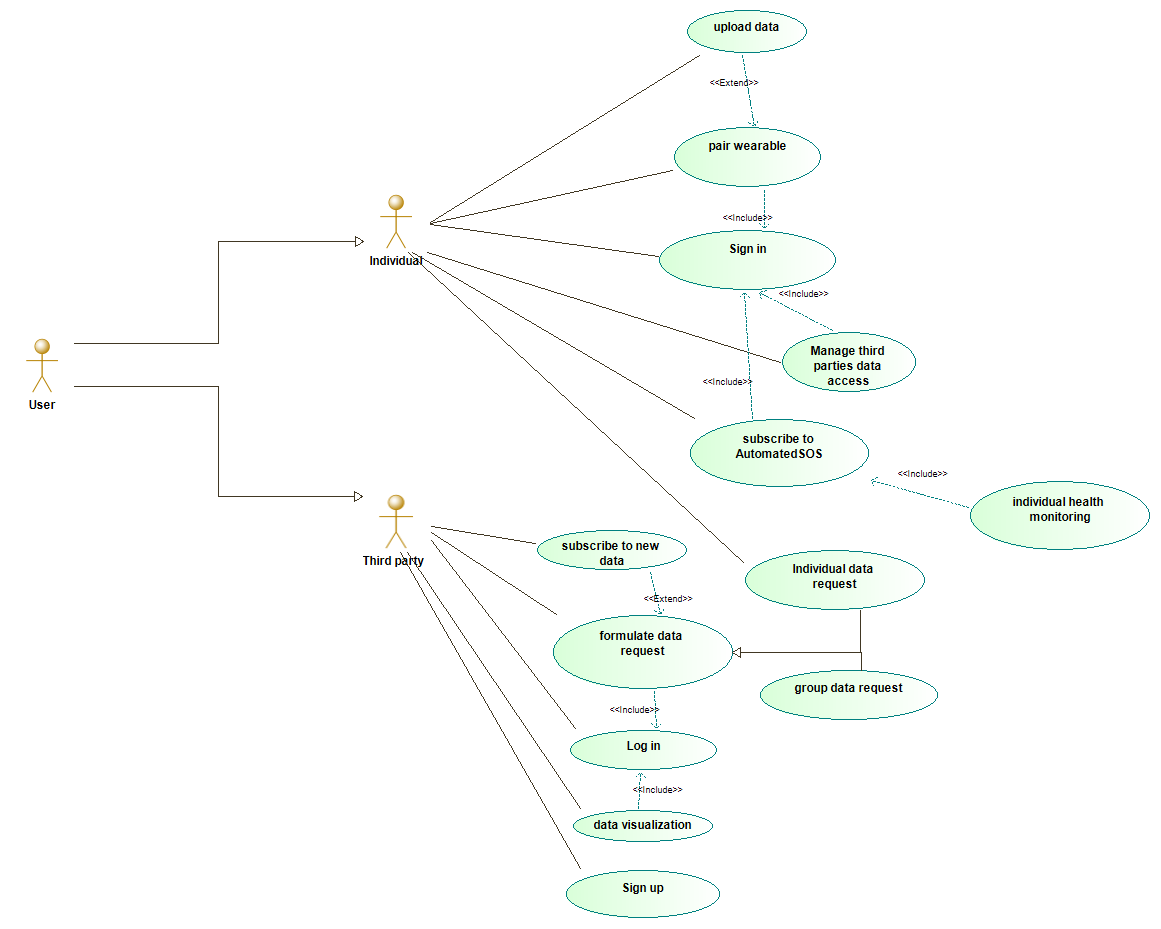
\includegraphics[width=1\linewidth]{resources/UML/GeneralUseCase.png}
  \caption{Data4Help Use case diagram}
  \label{fig:Use case diagram}
\end{figure}

\begin{table}[p]
\centering
\begin{tabular}{|l|p{11cm}|}
    \hline
    Name & Smartphone application sign up
    \\ \hline
    Actor & Individual
    \\ \hline 
    Entry condition & The individual installed the application and is connected to the internet
    \\ \hline
    Events flow &
    \begin{enumerate}
    \item The individual opens the application
    \item The individual taps on "Register a new account"
    \item The individual fills all the mandatory fields with correct information
    \item The individual clicks on "Register".
    \end{enumerate}
     \\ \hline
     Exit Condition & Individual credentials have successfully been added to the system,
     the individual can now log in     
     \\
    \hline
    Exceptions &
        \begin{enumerate}
    \item The individual username or his email is already present in the system database.
    \item Individual didn't fill all the mandatory fields.
    \item Individual provided invalid data.
    \end{enumerate}
    All the exceptions above are notified to the individual who is taken back to the registration form.
      \\
    \hline
\end{tabular}
\end{table}

\begin{table}[p]
\centering
\begin{tabular}{|l|p{11cm}|}
    \hline
    Name & Web application sign up
    \\ \hline
    Actor & Third party
    \\ \hline 
    Entry condition & The third party downloaded the web application and is connected to the internet
    \\ \hline
    Events flow &
    \begin{enumerate}
    \item The third party clicks on "Register a new account"
    \item The third party fills all the mandatory fields with correct information
    \item The third party clicks on "Sign up".
    \end{enumerate}
     \\ \hline
     Exit Condition & Third party credentials have successfully been added to the system,
     the third party can now log in     
     \\
    \hline
    Exceptions &
        \begin{enumerate}
    \item The third party username or his email is already present in the system database.
    \item The third party didn't fill all the mandatory fields.
    \item The third party provided invalid data.
    \end{enumerate}
    All the exceptions above are notified to the third party, which is taken back to the registration form.
      \\
    \hline
\end{tabular}
\end{table}

\begin{table}[p]
\centering
\begin{tabular}{|l|p{11cm}|}
    \hline
    Name & Smartphone Log In
    \\ \hline
    Actor & Individual
    \\ \hline 
    Entry condition & The individual has already signed up, has installed the application and is connected to the internet.
    \\ \hline
    Events flow &
    \begin{enumerate}
    \item The individual opens the application
    \item The individual fills the username and password field in the app homepage.
    \item The individual taps on "Log in".
    \item The username and the password inserted are sent to the system.
    \item The system checks if the credentials are valid.
    \end{enumerate}
     \\ \hline
     Exit Condition & The individual is successfully logged in and the app redirect him to the wearable pairing screen.
     \\
    \hline
    Exceptions &
	The inserted credentials are not found in the system database.
   The application notifies that the inserted credentials are wrong.
      \\
    \hline
\end{tabular}
\end{table}

\begin{table}[p]
\centering
\begin{tabular}{|l|p{11cm}|}
    \hline
    Name & Web application Log In
    \\ \hline
    Actor & Third party
    \\ \hline 
    Entry condition & The third party has already signed up, has downloaded the web application and is connected to the internet.
    \\ \hline
    Events flow &
    \begin{enumerate}
    \item The third party fills the username and password field in the web application homepage
    \item The third party clicks on "Log in".
    \item The username and the password inserted are sent to the system.
    \item The system checks if the credentials are valid.
    \end{enumerate}
     \\ \hline
     Exit Condition & The third party is successfully logged in and can access his personal area.
     \\
    \hline
    Exceptions &
    The inserted credentials are not found in the system database.  
   The application notifies that the inserted credentials are wrong.
      \\
    \hline
\end{tabular}
\end{table}


\begin{table}[p]
\centering
\begin{tabular}{|l|p{11cm}|}
    \hline
    Name & Wearable pairing
    \\ \hline
    Actor & Individual
    \\ \hline 
    Entry condition & The individual has logged in and both his wearable and his phone have bluetooth on.
    \\ \hline
    Events flow &
    \begin{enumerate}
    \item The individual reaches the wearable pairing screen.
    \item The individual ensures that the wearable is on and close to the smartphone.
    \item The individual taps on pair wearable.
    \end{enumerate}
     \\ \hline
     Exit Condition & Individual wearable is paired and the app is ready to gather individual eHealth data through it.
     \\
    \hline
    Exceptions &
        \begin{enumerate}
    \item The application isn't able to recognize a wearable. 
   	\item Bluetooth goes down during the pairing.
    \end{enumerate}
    The exception above is notified by the application. The individual can repeat the pairing procedure.
      \\
    \hline

\end{tabular}
\end{table}


\begin{table}[p]
\centering
\begin{tabular}{|l|p{11cm}|}
    \hline
    Name & Upload Data
    \\ \hline
    Actor & Individual
    \\ \hline 
    Entry condition & The individual is logged in and the wearable is paired.
    \\ \hline
    Events flow &
    \begin{enumerate}
    \item The wearable has gathered some individual eHealth data.
    \item The individual goes to the home application screen.
    \item The application downloads the data from the wearable.
    \item The application uploads the data on the system.
    \end{enumerate}
     \\ \hline
     Exit Condition & Individual eHealth data is successfully uploaded and stored in the system
     \\
    \hline
    Exceptions &
    \begin{enumerate}
    \item Connection falls down during the upload phase.
    \item The application fails the download of eHealth data from the individual's wearable. 
    \end{enumerate}
  The application notifies that there were problem during the upload phase. The individual can repeat the procedure by swiping down.
      \\
    \hline
\end{tabular}
\end{table}


\begin{table}[p]
\centering
\begin{tabular}{|l|p{11cm}|}
    \hline
    Name & Visualize data
    \\ \hline
    Actor & Individual
    \\ \hline 
    Entry condition & The individual is logged in and has already uploaded some data to the system
    \\ \hline
    Events flow &
    \begin{enumerate}
    \item The individual goes to "My data" section.
    \item The individual selects which data he wants to see in details.
    \item The application downloads the data from the system.
    \end{enumerate}
     \\ \hline
     Exit Condition & Individual eHealth data is successfully loaded on the device screen.
     \\
    \hline
    Exceptions &
    \begin{enumerate}
    \item Connection falls down during the upload phase.
    \item The application fails the download of eHealth data.
    \end{enumerate}
  The application notifies that there were problem during the upload phase. The individual can repeat the procedure by selecting again the data.
      \\
    \hline
\end{tabular}
\end{table}

\begin{table}[p]
\centering
\begin{tabular}{|l|p{11cm}|}
    \hline
    Name & Accept third parties data access requests.
    \\ \hline
    Actor & Individual, Third party
    \\ \hline 
    Entry condition & The individual is logged in and a data access request notification from a third party is received.
    \\ \hline
    Events flow &
    \begin{enumerate}
	\item The individual goes to the third parties access app section.
    \item The individual answers the data access request, giving or not giving the permission to the third party to access his data.
    \item The application forward the individual response to third party.
    \end{enumerate}
     \\ \hline
     Exit Condition & The third party is notified about the individual decision.
     \\
    \hline
    Exceptions &
        \begin{enumerate}
    \item Connection falls down while the individual is answering the request.
    \end{enumerate}
The application notifies that the device is disconnected.
      \\
    \hline
\end{tabular}
\end{table}


\begin{table}[p]
\centering
\begin{tabular}{|l|p{11cm}|}
    \hline
    Name & Remove third parties data access
    \\ \hline
    Actor & Individual
    \\ \hline 
    Entry condition & The individual is logged in and wants to remove a third party data access
        \\ \hline
    Events flow &
    \begin{enumerate}
	\item The individual goes to the third parties management app section.
    \item The individual clicks on the remove button associated to the third party.
    \end{enumerate}
     \\ \hline
     Exit Condition & The system correctly change data access permissions and notifies the third party of the change
     \\
    \hline
    Exceptions &
        \begin{enumerate}
    \item No third party already has access to individual's data. The app notifies the individual about it.
    \item The connection goes down during the process. The app notifies this to the individual, who will have to repeat the procedure when the connection is back.
    \end{enumerate}
       \\
    \hline
\end{tabular}
\end{table}


\begin{table}[p]
\centering
\begin{tabular}{|l|p{11cm}|}
    \hline
    Name & Subscribe to AutomatedSOS service
    \\ \hline
    Actor & Individual
    \\ \hline 
    Entry condition & The individual is logged in and the wearable is paired
        \\ \hline
    Events flow &
    \begin{enumerate}
	\item The individual goes to the AutomatedSOS app section.
    \item The individual click the subscribe button.
    \item The app checks if the wearable paired can gather the necessary data for the AutomatedSOS service.
    \item The app starts monitoring the individual.
    \end{enumerate}
     \\ \hline
     Exit Condition & The wearable starts monitoring individuals vital parameters
     \\
    \hline
    Exceptions &
        \begin{enumerate}
    \item Wearable cannot monitors individuals vital parameters.
    \item Wearable unpairs during the procedure.
    \item The connection falls down during the procedure.
    \end{enumerate}
      The exception above are notified to the individuals. The individual must repeat the whole 
      procedure.
      \\
    \hline
\end{tabular}
\end{table}

\begin{table}[p]
\centering
\begin{tabular}{|l|p{11cm}|}
    \hline
    Name & Individual data request
    \\ \hline
    Actor & Third party
    \\ \hline 
    Entry condition & The third party is logged in and knows the individual's username or TC
        \\ \hline
    Events flow &
    \begin{enumerate}
    \item The third party selects the data request button.
	\item The third party insert the individual identifier (either his username or his TC).
	\item The system forwards the request to the individual.
    \end{enumerate}
     \\ \hline
     Exit Condition & A notification of a new data access request is sent to the individual
     \\
    \hline
    Exceptions &
        \begin{enumerate}
    \item The individual identifier is not found in the system.
    \end{enumerate}
     The exception above is notified to the third party, which is sent back to the data request screen.
        \\  \hline

\end{tabular}
\end{table}


\begin{table}[p]
\centering
\begin{tabular}{|l|p{11cm}|}
    \hline
    Name & Group data request
    \\ \hline
    Actor & Third party
    \\ \hline 
    Entry condition & The third party is logged in
        \\ \hline
    Events flow &
    \begin{enumerate}
    \item The third party goes in the data request section.
    \item The third party selects the group data request.
	\item The third party can apply filters on his request. To be precise it can filter data by individuals age, sex, location (country, city) and can specify which data it is interested in (steps taken ,sleep hours, average heart rate, average blood pressure). The time interval of the each requested data can be specified.
	\item The system analyzes the request and distributes the requested data to the third party.
    \end{enumerate}
     \\ \hline
     Exit Condition & The requested data is visualized by the third party
     \\
    \hline
    Exceptions &
        \begin{enumerate}
    \item The group of individuals detected by the third party has a number of members of 1000 or less.
    \end{enumerate}
      The exception above is notified to the third party, which is sent back to the data request screen.
	 \\
    \hline
\end{tabular}
\end{table}

\begin{table}[H]
\centering
\begin{tabular}{|l|p{11cm}|}
    \hline
    Name & Visualize data
    \\ \hline
    Actor & Third party
    \\ \hline 
    Entry condition & The third party is logged in and has access to some data (either group or individual)
        \\ \hline
    Events flow &
    \begin{enumerate}
    \item The third party goes in the data visualization section.
	\item The third party clicks on the subscribe button of the data request he is interested in.
	\item The system starts automatically to update the data to which the third party is subscribed to.
    \end{enumerate}
     \\ \hline
     Exit Condition & The application notifies the third party of the new subscription.
     \\
    \hline
    Exceptions &
        \begin{enumerate}
    \item The number of individuals of the group detected by the data request which the third party wants to subscribe to went to 1000 or below.
    \item The individual removed the permission to access his data from the third party.
\end{enumerate}  
 The exceptions above are notified to the third party that will not be updated anymore with new data.
  \\
    \hline
\end{tabular}
\end{table}



\subsection{Sequence diagrams}
The following diagrams model the main features of Data4Help: data uploading by individuals, data request by third parties and AutomatedSOS subscription.
Some assumptions were considered in order to simplify these diagrams, the system should act without them:
\begin{itemize}
\item The login credentials provided by the users are correct;
\item The wearable used during the pairing is compatible with the applications;
\item User devices are connected to the internet for the whole time.
\end{itemize}





\begin{figure}[p]
	\centering
  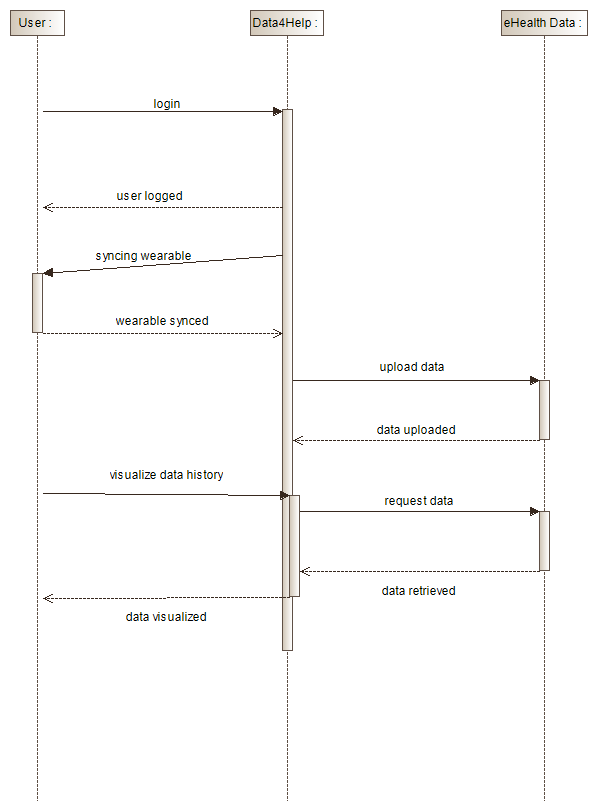
\includegraphics[width=0.79\linewidth]{resources/UML/IndividualInteraction.png}
  \caption{Individual data upload screen}
  \label{fig:Individual sequence diagram}
\end{figure}

\begin{figure}[p]
	\centering
  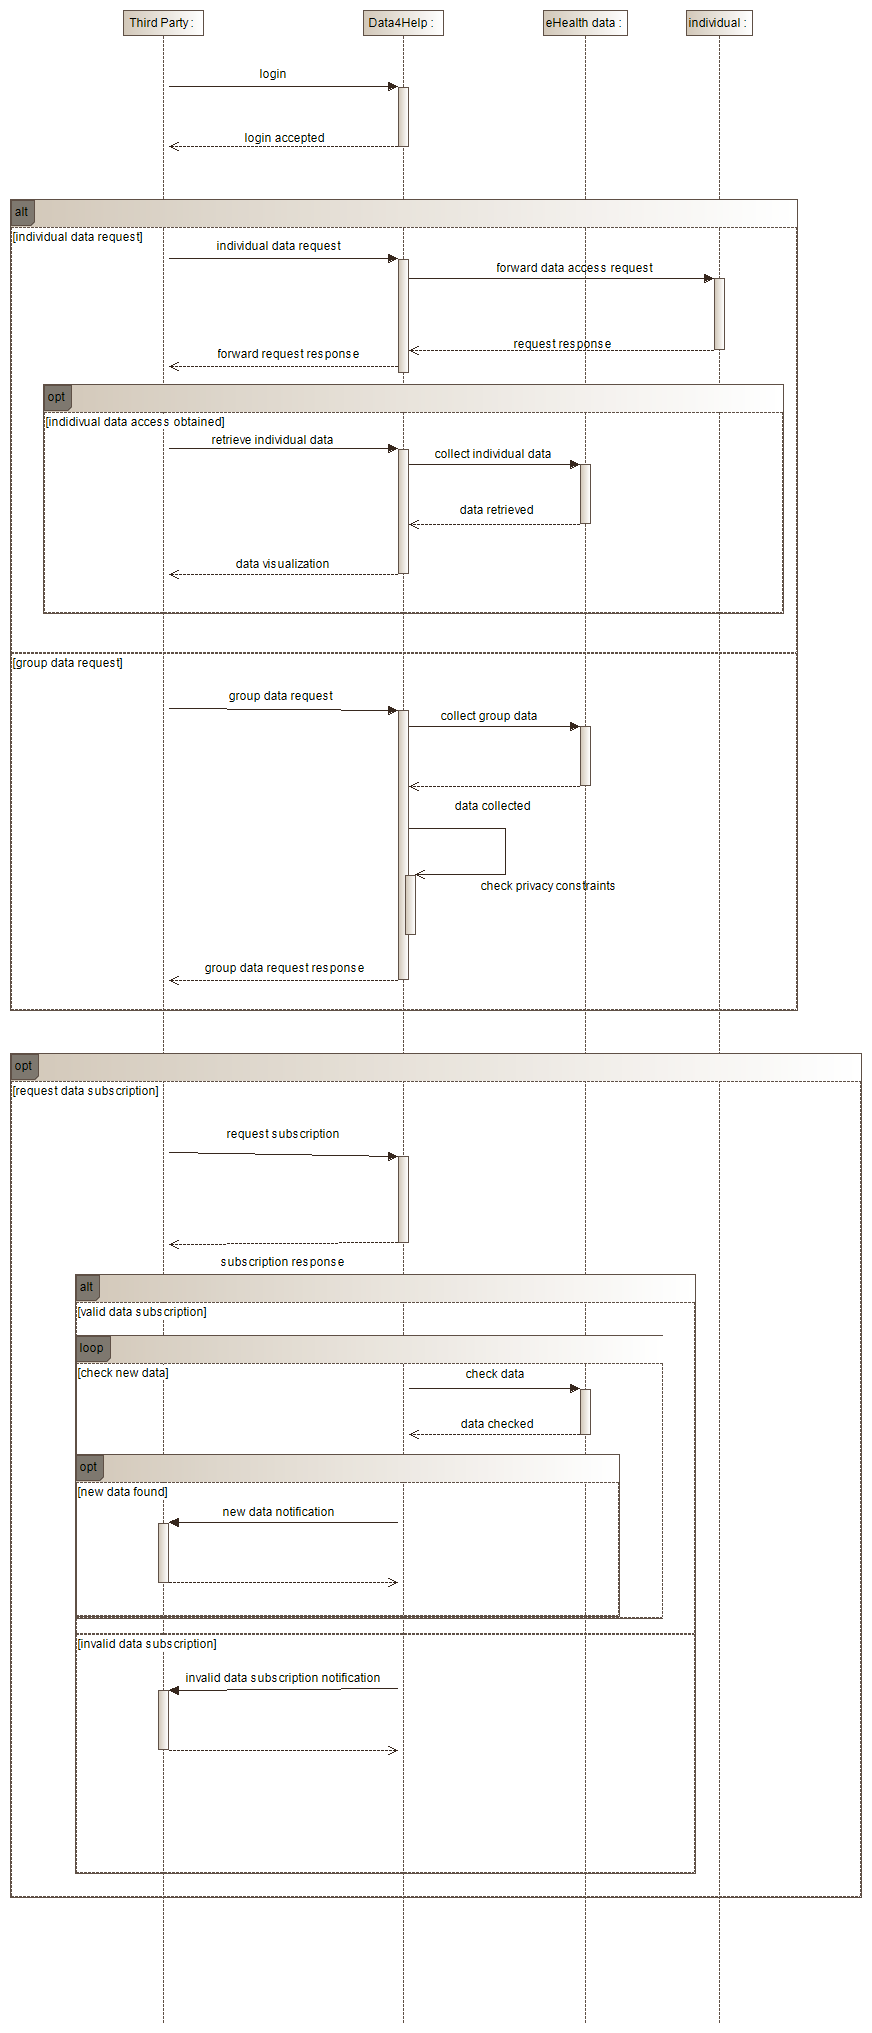
\includegraphics[width=0.67\linewidth]{resources/UML/ThirdPartyDataRequest.png}
  \caption{Third Party data request sequence diagram}
  \label{fig: ThirdParty sequence diagram}
\end{figure}

\begin{figure}[H]
	\centering
  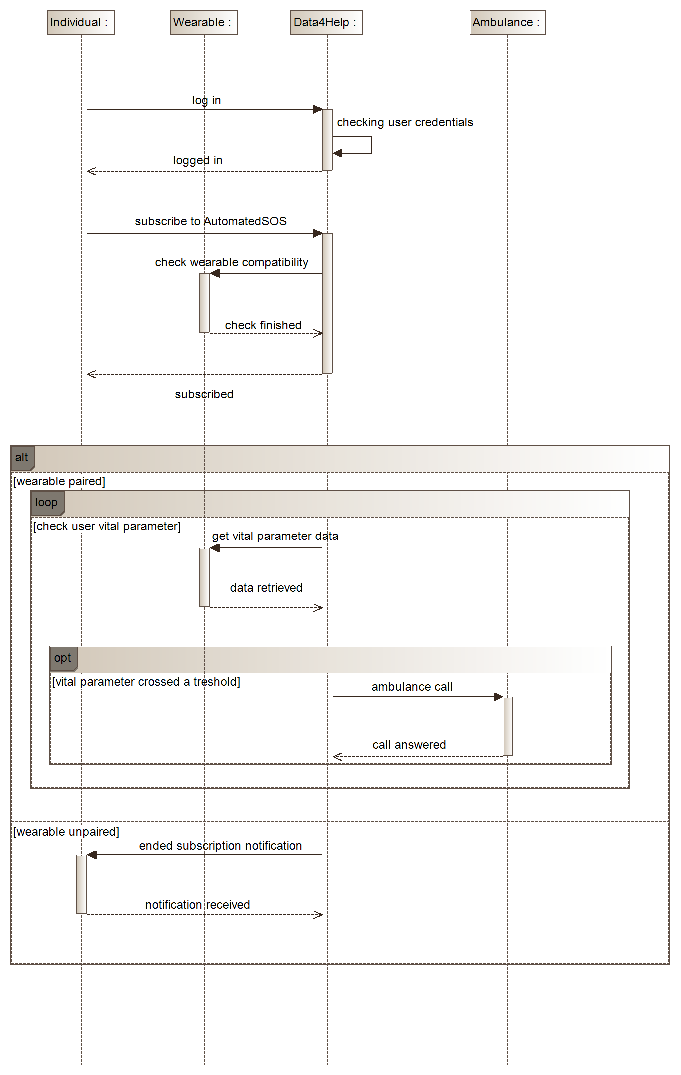
\includegraphics[width=0.70\linewidth]{resources/UML/AutomatedSOSsequence.png}
  \caption{AutomatedSOS subscription sequence diagram}
  \label{fig: AutomatedSOS sequence diagram}
\end{figure}



\section{Performance Requirements}
Data4Helps is a service that strongly depends on the amount of data gathered, therefore the initial phase will focus on recruiting as more individuals as possible.

Giving a realistic estimation on the numbers of users is not possible but a total amount of 100000 individuals and 500 third parties will be considered a good starting point.

In order to expand the user base and have from the start good feedback the development will be focused on providing a reliable and persistent service. 

Regarding the AutomatedSOS service, the ambulance call should be done with a delay time from the crossing of the critical thresholds that is under 5 seconds.

\section{Design constraints}
\subsection{Standards compliance}
\begin{itemize}
\item The app only requests the minimum permissions in order to guarantee its core functionalities: storage access, location and wearable access.
\item The app only supports portrait mode.
\item All the data gathered through individuals wearables will be uploaded and stored in the system database.
\end{itemize}


\subsection{Hardware limitations}
Individuals will use a smartphone app in order to access the service.
The following devices are the one that will be compatible with the app:
\begin{itemize}
\item Android smartphone with following capabilities:
\begin{itemize}
\item 2G/3G/4G connection;
\item Bluetooth connection;
\item GPS;
\end{itemize}

These are instead the smartwatches that will be initially supported in the app:
\item watchOS or wearOS smartwatch


Third parties will have access to the service through a WebApp, accessible with any browser compatible with html5 and java.
\end{itemize}

\subsection{Other constraints}
The app must make clear that \textbf{AutomatedSOS service DOES NOT substitute} the manual emergency call since that the availability of the service rely on external factors such as internet connection, wearable hardware and only a couple of vital parameters can be monitored.


The Automated SOS service was born as an additional service that can anticipate the emergency call, not as a service that substitutes it.


\section{Software system constraints}
\subsection{Reliability}
The application aims to provide a 24/7 service, but, especially in the initial phase, some time of unavailability for maintenance is expected.
\subsection{Availability}
The initial target of availability will be a system that is up for the 95.00\% of the time. This value should improve over time as the service expands and more resources are available.
\subsection{Security}
Users passwords will be encrypted and stored in a specific database.
\subsection{Mantainability}
The whole system will be designed in a modular way in order to separate each component from the other ones, guaranteeing an high level of flexibility. 

AutomateSOS is a first, clear example of the expandability nature of Data4Help.
\subsection{Compatibility}
Gathering the possible largest amount of eHealth data is the fundamental feature of the service. Although, due the fragmentation of the wearable market and limited resources, only wearOS smartwatches will be initially supported. 


The app will support Android smartphones while the WebApp will be compatible with any browser that supports html5 and java applets.


Since Data4Help aims to acquire the largest amount of data, other smartphones and smartwatches may be considered in the future for a port of the application.


\subsection{Portability}
In order to optimize resources the application will be initially only developed for Android and wearOS smartwatches.

Since Data4Help strongly relies on the amount of its registered individuals, any operative system that has at least 10\% share of the market will be considered for an application port.
